\section{Hagan Rowlenstino/1174040}
	\subsection{Soal 1} 
		\begin{itemize}
			\item Device Manager : Seperti namanya sendiri, device manager berfungsi untuk menampilkan dan mengelola semua hardware yang terinstall ataupun dapat di instalasi ke dalam windows.

			\item folder /dev : Di dalam sistem operasi Linux, perangkat yang tehubung akan dianggap sebagai file. di dalam folder /dev inilah file - file  tersebut berada.
		\end{itemize}

	\subsection{Soal 2}
	Langkah - langkah instalasi driver arduino :
		\begin{enumerate}
			\item download file driver arduino terlebih dahulu dan masukkan ke dalam directory yang diinginkan
			\item hubungkan arduinio uno anda ke pc anda dengan kabel USB yang tersedia
			\item lalu windows akan memunculkan pop up yang memberitahu bahwa ingin menginstall dirver, tapi nanti tidak akan menemukan drivernya
			\item buka Device Manager 
			\item cari unknown device di dalam Device Manager di dalam tab other device
			\item klik kanan pada unknown device tersebut lalu pilih update driver software
			\item pilih browse my computer for driver software lalu masukkan directory dimana anda menyimpan driver arduino yang telah anda download tadi
			\item setelah itu klik install dan tunggu hingga proses selesai
			\item arduino pun sudah terbaca di pc anda 
		\end{enumerate}

	\subsection{Soal 3}
	Untuk melihat atau membaca baudrate dan port kita hanya perlu menginstall Arduino IDE, setelah itu buka menu serial monitor yang berada di tab tools. Dari sana akan terlihat baik baudrate dan port yang sedang digunakan oleh arduin anda.

	\subsection{Soal 4}
	PySerial merupakan sebuah library yang digunakan untuk komunikasi ke port serial terutama untuk mikrokontroller. PySerial pertama kali diluncurkan pada tahun 2002 yang makin berkembang dalam setiap versinya hingga tahun 2017 lalu.

	\subsection{Soal 5}
		\begin{itemize}
			\item \begin{verbatim}stop()\end{verbatim} : untuk menghentikan pembacaan program
			\item \begin{verbatim}serial.to_bytes(sequence)\end{verbatim} : berfungsi untuk mengubah sequence ke dalam bytes agar dapat dikirim ke dalam arduino.
			\item \begin{verbatim}close()\end{verbatim} : untuk menutup port dan menghentikan pembacaan program
		\end{itemize}

	\subsection{Soal 6}
	Dengan menggunakan pengulangan kita dapat mengambil data berkali - kali tanpa harus mengeksekusi file python tersebut berulang - ulang. Tanpa perulangan juga penting karena dapat digunakan di saat saat tertentu seperti jika ingin mengukur suhu ruangan yang hanya dilakukan pada saat saat tertentu tidak terus menerus.

	\subsection{Soal 7}
	Untuk membuat fungsi yang menggunakan pyserial kita hanya perlu untuk menginisialisasi pembubatan funsi dengan menggunakan def namafungsi() : lalu masukkan pyserial tersebut dengan indentasi. atau cukup dengan menggunakan fungsi while loop degan menggunakan while true:
	
\section{Luthfi Muhammad Nabil/1174035}
\subsection{Soal 1}
Apa itu fungsi device manager di windows dan /dev di linux :
\begin{itemize}
	\item Device Manager merupakan panel kontrol pada sistem operasi windows. Pengguna dapat mengontrol dan melihat perangkat yang  telah terhubung dengan komputer dengan device manager. 
	Untuk setiap perangkat, pengguna dapat : 
		\begin{itemize}
			\item Memperbolehkan perangkat untuk beroperasi
			\item Menginformasikan sistem operasi untuk melakukan aksi pada perangkat yang tidak berfungsi
			\item Menginstall driver untuk perangkat yang terhubung
			\item Melihat informasi dari perangkat
		\end{itemize}
	\item /dev merupakan lokasi dari file untuk perangkat. /dev berfungsi untuk menampung data - data sebuah perangkat yang terhubung pada komputer. Perangkat yang dapat terhubung diantaranya perangkat penyimpanan data dan perangkat pengiriman data.
\end{itemize}

\subsection{Soal 2}
Jelaskan langkah - langkah instalasi driver dari arduino : 

Untuk instalasi driver, biasanya akan langsung terinstall jika sudah menginstall arduino IDE Seperti contoh meminta instalasi untuk arduino pada gambar \ref{PopUpInstalasi}.
\begin{figure} [ht]
		\centerline{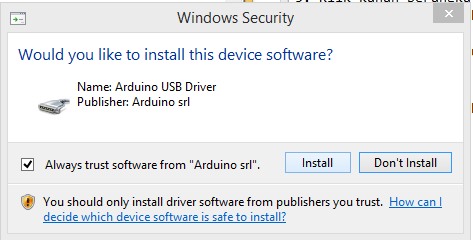
\includegraphics[width=1\textwidth]{figures/5/1174035/Teori/PopUpInstalasi.png}}
		\caption{Pop Up saat instalasi Arduino IDE}
		\label{PopUpInstalasi}
\end{figure}
Jika memang tidak ditemukan, maka ikuti langkah berikut : 
Yang dibutuhkan : 
\begin{itemize}
	\item Arduino Driver
	\item Arduino Jenis Apapun
\end{itemize}
Cara Instalasi : 
\begin{enumerate}
	\item Hubungkan arduino ke komputer (untuk arduino uno dapat menggunakan kabel type B)
	\begin{figure} [ht]
		\centerline{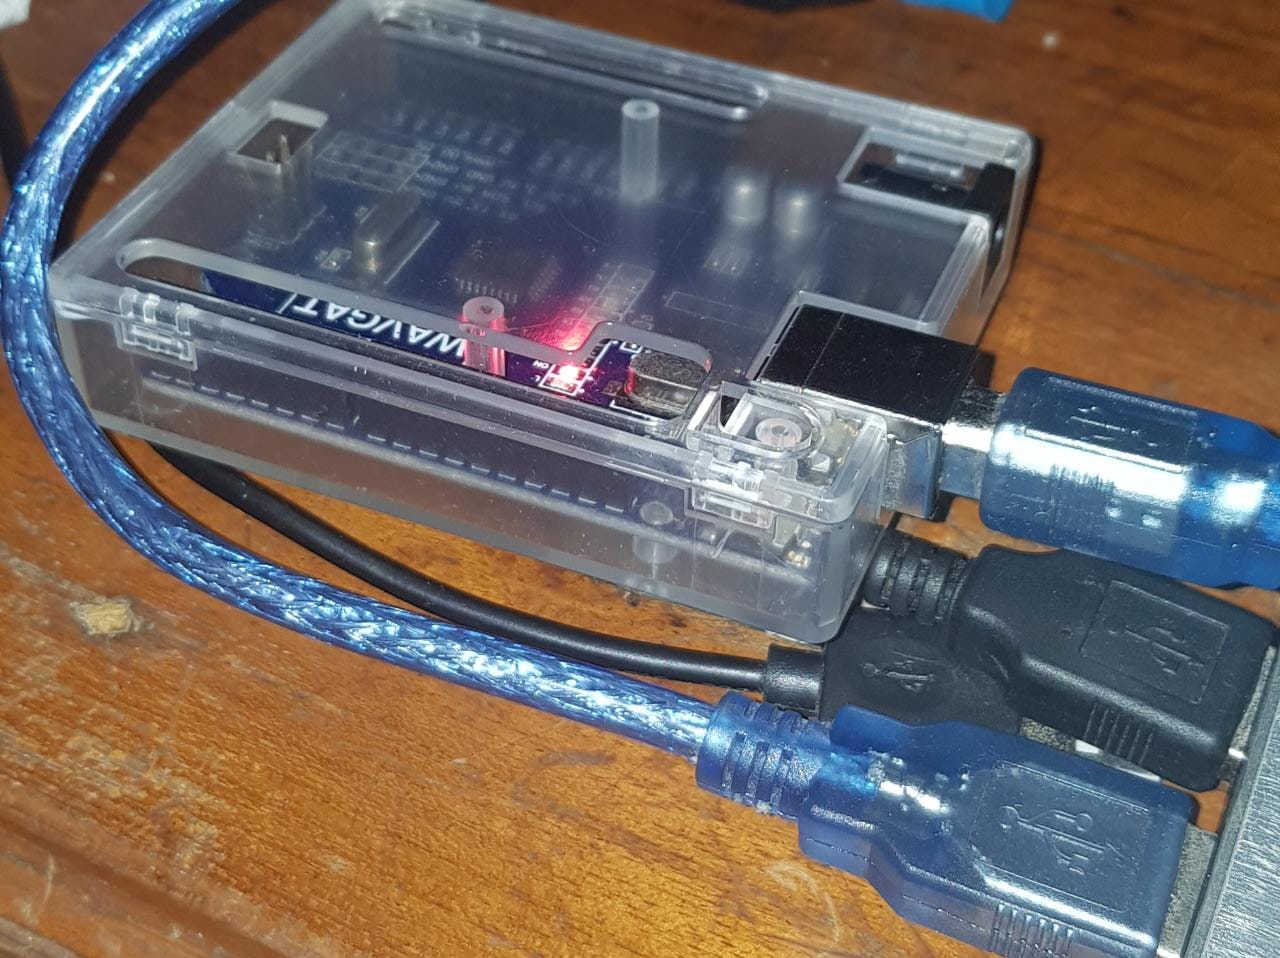
\includegraphics[width=0.6\textwidth]{figures/5/1174035/Teori/Soal1Step1.jpeg}}
		\caption{Hubungkan arduino dengan komputer}
		\label{Soal1Step1}
	\end{figure}
	\item Lalu setelah muncul popup instalasi driver akan terinstal secara otomatis. 
	\item Jika instalasi otomatis gagal, buka device manager.
		\begin{figure} [ht]
			\centerline{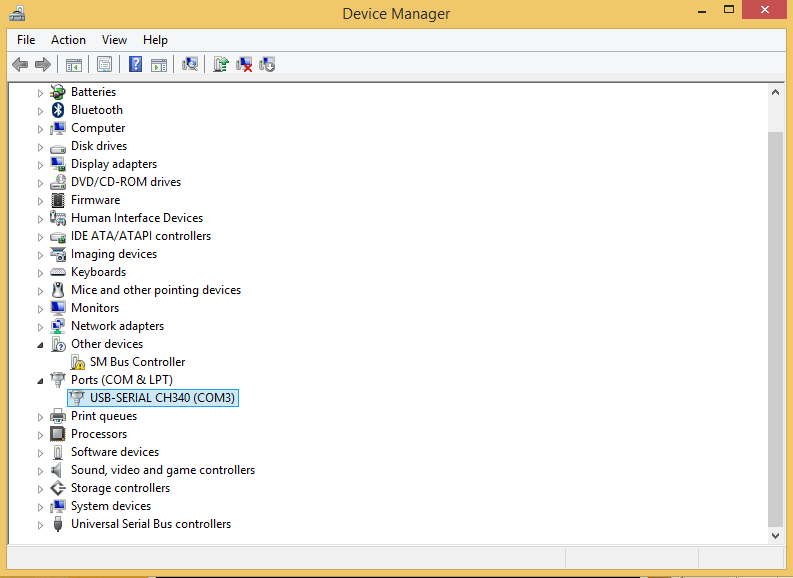
\includegraphics[width=1\textwidth]{figures/5/1174035/Teori/DeviceManagerContoh.png}}
			\caption{Tampilan Device Manager}
			\label{DevManagerContoh}
		\end{figure}
	\item Setelah device manager terbuka, cari perangkat lainnya/tidak diketahui (other device).
	\item Klik kanan perangkat yang tidak diketahui lalu pilih update driver.
	\item Pilih Cari driver (Browse my computer for driver software).
	\item Pilih lokasi driver ke driver yang telah didownload lalu klik next/ok.
	\item Setelah muncul pop up instalasi, tekan install.
	\item Instalasi Sukses
\end{enumerate}

\subsection{Soal 3}
Jelaskan bagaimana membaca baudrate dan port dari komputer yang sudah terinstall driver : 
\begin{itemize}
	\item Port : Untuk membaca port, dapat membuka file/lokasi berikut :
	
Arduino IDE : 
	\begin{figure} [ht]
			\centerline{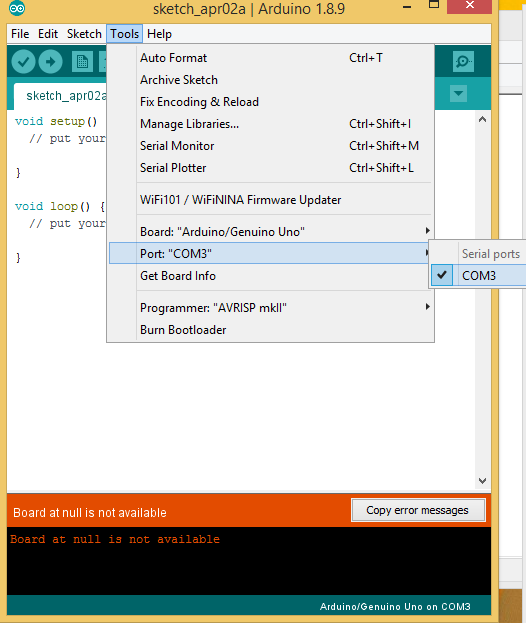
\includegraphics[width=0.6\textwidth]{figures/5/1174035/Teori/PortArduinoIDE.png}}
			\caption{Port dari Arduino IDE}
			\label{IDEPorts}
		\end{figure}
		\begin{enumerate}
			\item Buka Arduino IDE
			\item Lalu masuk ke Tools->Ports
			\item Akan muncul port serial untuk arduino seperti pada gambar \ref{IDEPorts}
		\end{enumerate}
Device Manager : 
	\begin{figure} [ht]
			\centerline{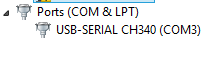
\includegraphics[width=0.6\textwidth]{figures/5/1174035/Teori/PortDeviceManager.png}}
			\caption{Port dari Device Manager}
			\label{DevManPort}
		\end{figure}
		\begin{enumerate}
			\item Buka Device Manager pada windows
			\item Cari Perangkat dengan nama Arduino
			\item Lalu lihat port berapa yang dipakai oleh Arduino Tersebut seperti pada gambar \ref{DevManPort}
		\end{enumerate}		
	\item Baudrate : Untuk melihat baudrate, dapat buka serial monitor dan cek baudrate dan tampilan fix pada tampilan serial monitor. Untuk setting default biasanya diantara 9600 dan 115200.
	\begin{figure} [ht]
			\centerline{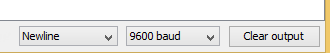
\includegraphics[width=0.6\textwidth]{figures/5/1174035/Teori/Baudrate.png}}
			\caption{Baud Rate}
			\label{BaudRate}
		\end{figure}
\end{itemize}

\subsection{Soal 4}
Sejarah PySerial : 

PySerial dibuat secara public pertama kali pada tahun 2002 dengan rilisan versi pertama 1.0. Pada saat itu PySerial sudah dapat membaca line serial dan menghapus semua isi dari serial tetapi belum dapat mengkonversi isi serial menjadi tipe data lain. PySerial juga sudah dapat melakukan Exception untuk proses yang terdapat error. Lalu pada tahun 2003 dirilis versi yang dapat mengkonversi data ke bilangan bulat, suppert terhadap python versi 2.2+ dan getter setter. Mulai pada tahun 2008, diberlakukan fitur iterasi untuk dapat mengambil seluruh data yang muncul pada serial yang diusulkan oleh Bernhard Bender. Kemudian pada tahun 2011, mulai dapat melihat daftar port yang terhubung dengan serial. Sampai akhirnya telah muncul versi 3.4 pada tahun 2017 yang sudah memperbaiki bug - bug yang ada.

\subsection{Soal 5}
Jelaskan fungsi - fungsi yang ada di pyserial.
\begin{itemize}
	\item \begin{verbatim}open()\end{verbatim} 
	Fungsi untuk membuka port serial yang terhubung
	\item \begin{verbatim}close()\end{verbatim} 
	Fungsi untuk menutup port serial yang terhubung
	\item \begin{verbatim}read(size=1) \end{verbatim}
	Fungsi untuk menentukan ukuran serial yang dapat dibaca
	\item \begin{verbatim}read\_until(expected=LF, size=None) \end{verbatim}
	Fungsi untuk membaca serial sampai sequence yang ditentukan sudah dapat.
	\item \begin{verbatim}write(data) \end{verbatim}
	Fungsi untuk menulis data ke perangkat yang terhubung.
	\item \begin{verbatim}flush() \end{verbatim}
	Fungsi untuk menghapus seluruh data yang ditampilkan di serial.
	\item \begin{verbatim}readline(size=-1) \end{verbatim}
	Untuk membaca setiap line pada tampilan yang ada pada serial
	\item \begin{verbatim}writelines(lines) \end{verbatim}
	Sama halnya dengan write yaitu untuk menulis data ke perangkat yang terhubung.
\end{itemize}
\subsection{Soal 6}
Jelaskan mengapa butuh perulangan dalam membaca serial : 

Karena perulangan digunakan untuk membaca seluruh data pada serial yang ada setiap baris. Perulangan digunakan agar data dapat muncul secara terus menerus atau realtime. Dalam konsep berjalannya sebuah microcontroller, proses yang ada akan dijalankan secara terus menerus sampai proses meminta atau processor meminta untuk memberhentikan proses tersebut sehingga jika tidak memakai perulangan, maka data yang diambil hanyalah data dimana sintaks untuk meminta data itu dipanggil. 
\subsection{Soal 7}
Jelaskan cara membuat fungsi yang menggunakan pyserial : 

Untuk membuat fungsi yang menggunakan pyserial, cukup dengan menuliskan fungsi dari pyserial dan menggunakannya dalam fungsi yang dibuat. Seperti contoh fungsi yang menggunakan PySerial : 
\lstinputlisting{src/5/1174035/Teori/chap5_1174035_teori.py}
